\documentclass[12pt]{article}

\usepackage{pablo-devoir}
\usepackage{pablo-listings}
\usepackage[a5paper,margin=2cm]{geometry}

\pagestyle{empty}

\title{(In)Équation\\Espace}
\date{10/11/14}
\classe{2\up{des}14}
\dsnum{DS 2 bis}

\begin{document}

\maketitle

\begin{exercice}[Développement et Factorisation --- 6 points]
  On considère la fonction définie par $f(x)=\left( 2x-1 \right)\left( 2x+5 \right)$.

  \begin{enumerate}[(1)]
    \item
      \begin{enumerate}
        \item Montrer que $f(x)=4x^2+8x-5$.
        \item Montrer que $f(x)=(2x+2)^2-9$.
      \end{enumerate}
    \item \begin{enumerate}
        \item Résoudre $f(x)=-9$.
        \item Résoudre $f(x)=-5$.
      \end{enumerate}
  \end{enumerate}
\end{exercice}

\begin{exercice}[Inéquations --- 6 points]
  Résoudre (si nécessaire) les inéquations suivantes, et présenter les solutions sur la droite des réels, puis sous forme d'intervalle.
  \begin{enumerate}[(1)]
    \item $2+5x>3x-4$
    \item $x<2$ ou $x>0$
    \item $x<2$ et $x>0$
  \end{enumerate}
\end{exercice}

\pagebreak

\begin{exercice}[Volume --- 6 points]~
  \begin{multicols}{2}
    Un cylindre de révolution est inscrit dans un cône de révolution, comme dans la figure ci-contre.

    Le cône fait 20~cm de hauteur, et sa base a un rayon de 8~cm.

    La hauteur du cylindre est la moitié de celle du cône ; le rayon de la base du cylindre est la moitié du rayon de la base du cône.

    \columnbreak

    \begin{center}
      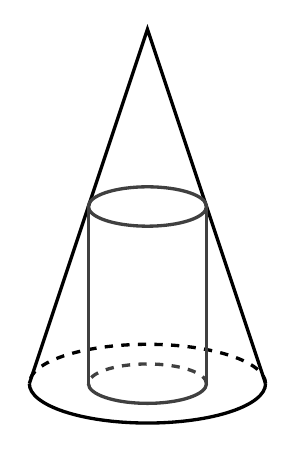
\begin{tikzpicture}[very thick,scale=.5]
        \draw[] (0,0) -- (3, 9) -- (6,0);
        \draw[] (0,0) arc (180:360:3 and 1);
        \draw[dashed] (6,0) arc (0:180:3 and 1);

        \draw[darkgray,] (1.5,0) arc (180:360:1.5 and .5);
        \draw[darkgray,dashed] (4.5,0) arc (0:180:1.5 and .5);
        \draw[darkgray,] (1.5, 0) -- ++(0,4.5);
        \draw[darkgray,] (4.5, 0) -- ++(0,4.5);
        \draw[darkgray,] (3,4.5) ellipse (1.5 and 0.5);
      \end{tikzpicture}
    \end{center}
  \end{multicols}

  Les résultats seront arrondis à l'unité.

  \begin{enumerate}
    \item Calculer le volume du cône.
    \item Calculer le volume du cylindre.
    \item Le volume du cylindre est-il plus petit ou plus grand que la moitié du volume du cône ?
  \end{enumerate}


\end{exercice}

\begin{exercice}[Problème ouvert --- 2 points]\emph{Toute trace de recherche, même incomplète, sera prise en compte dans la notation.}
  \begin{multicols}{2}
    \noindent Pour aller du point $A$ au point $G$ sur le cube ci-contre, de 10~cm de côté, une fourmi passe par le point $I$, milieu de $[BF]$.

    Quelle distance a-t-elle parcouru ?

    \begin{center}
      \begin{tikzpicture}[scale=2, thick]
        \coordinate (O) at (0,0);
        \coordinate (x) at (1,0);
        \coordinate (y) at ({0.8*cos(35)},{0.8*sin(35)});
        \coordinate (z) at (0,1);

        \coordinate (A) at (O);
        \coordinate (B) at ($(O) + (x)$);
        \coordinate (C) at ($(O) + (x) + (y)$);
        \coordinate (D) at ($(O) + (y)$);
        \coordinate (E) at ($(O) + (z)$);
        \coordinate (F) at ($(O) + (z) + (x)$);
        \coordinate (G) at ($(O) + (z) + (x) + (y)$);
        \coordinate (H) at ($(O) + (z) + (y)$);
        \coordinate (I) at ($(O) + 0.5*(x) + 0.5*(z)$);
        \coordinate (J) at ($(O) + (x) + 0.5*(y) + 0.5*(z)$);

        \draw (A) node[below left]{$A$};
        \draw (B) node[below right]{$B$};
        \draw (C) node[right]{$C$};
        \draw (D) node[above left]{$D$};
        \draw (E) node[left]{$E$};
        \draw (F) node[above]{$F$};
        \draw (G) node[right]{$G$};
        \draw (H) node[above]{$H$};
        \draw (A) -- (B) -- (C) -- (G) -- (H) -- (E) -- (F) -- (B);
        \draw (A) -- (E);
        \draw (F) -- (G);
        \draw[dashed] (D) -- (H);
        \draw[dashed] (D) -- (A);
        \draw[dashed] (D) -- (C);

        \coordinate (I) at ($(O) + (x) + 1/2*(z)$);

        \draw[ultra thick, gray] (A) -- (I) -- (G);
        \draw (I) node[right]{$I$};

      \end{tikzpicture}
    \end{center}
  \end{multicols}
\end{exercice}
\end{document}
